\PassOptionsToClass{final}{JHD}
\documentclass{JHD}
\usepackage{bm}
\usepackage{tabularray}
\usepackage{amsmath}
%\Year{2025}
%\Vol{37}
%\No{4}
%\StartPage{664}
%\EndPage{679}
%\DOI{10.1007/s42241-025-0025-2}
%\DateInfo{(Received January 9, 2025, Revised January 17, 2025, Accepted January 18, 2025, Published online October 20, 2025)}
\RightsInfo{\textcopyright{} China Ship Scientific Research Center 2026}
\BeginPage{666}
\begin{document}
\title{Demonstrative Material and Its Application in the Prototyping and Validation of Scholarly Journal Formatting Specifications}
\author{
John Q. Sample\an{1},
Jane A. Placeholder\an{1,2},
Max D. Dummy\an{1,3*},
Alice T. Testcase\an{2,3},
Robert L. Filler\an{1,2,3}
}
\affiliation{
1. Department Affiliation, School or Company Affiliation, City, State, postcode, country\\
2. Department Affiliation, School or Company Affiliation, City, State, postcode, country\\
3. Department Affiliation, School or Company Affiliation, City, State, postcode, country
}
\ExtraInfo{
Project supported by the XXX Foundation (Grant No. XXXXXXXX).\\
\textbf{Biography:} Author Name (1990--), Gender, Academic Degree,\\
E-mail: placeholder.email@example.com\\
\textbf{Corresponding author:} Author Name,\\
E-mail: corresponding.author@example.com
}
\abstract{
This abstract outlines a placeholder framework for template demonstration. The core concept is derived from a basic expression $y=f(\theta,x)$, where $\theta$ denotes a parameter set and $x$ an input variable. A common constraint $g(x)\leq C$ is often applied, with $C$ being a constant threshold. The performance metric $\eta=S/N$ is used for illustration, where $S$ and $N$ represent generic signal and noise terms, respectively. The discussion herein is purely structural and contains no substantive claims.
}
\keywords{placeholder text, template demonstration, sample content, structural preview, formatting example}
\maketitle
\section{Introduction}
This introductory section presents a placeholder discussion on template formatting. The primary objective is to demonstrate the visual integration of mathematical expressions within text. Consider a generic relation $z = \alpha x + \beta y$, where $\alpha$ and $\beta$ are placeholder coefficients. For the purpose of layout demonstration, the continuity equation is also provided:
\begin{equation}
 \frac{\partial \rho }{\partial t} +\nabla\ \cdot (\rho \bm U)=0
\end{equation}
\par
The equation above serves no analytical role and is included purely for structural visualization.
\par
A subsequent illustrative paragraph is included to show text flow around a displayed equation. In most placeholder contexts, a standard form such as $p \propto \exp(-E/k)$ may be referenced. To further exemplify formatting,  the momentum equation is presented:
\begin{equation}
 \frac{\partial \rho \bm U}{\partial t} + \nabla\ \cdot (\rho \bm U  \bm U) = -\nabla\ p + \rho \bm g + \nabla\ \cdot (\mu \nabla\  \bm U )
\end{equation}
\par

All symbols in the preceding equations are devoid of semantic meaning.
\par
Finally, a concluding placeholder remark is offered. One might define a simple ratio $R = A/B$ to represent an arbitrary quantity. For completeness, the energy equation is shown:
\begin{equation}
	\begin{split}
		&  c_v[\frac{\partial\rho T}{\partial t} + \nabla \cdot (\rho \bm U T)]\\
		& = -  \nabla \cdot (p \bm U )-\frac{2}{3} \mu ( \nabla \cdot \bm U )+2 \mu \bm S : \bm S +  \nabla \cdot (k \nabla T )
	\end{split}
\end{equation}
\par
The entire content of this section, including all formulas, is intended solely for template preview purposes and carries no technical significance.
\section{Methodology and Framework Overview}
This section provides a descriptive overview of the placeholder methodology employed in this template demonstration. The primary aim is to illustrate the structural organization of a typical research manuscript, encompassing various levels of headings and the integration of visual elements. A fundamental assumption in this illustrative framework is that a placeholder variable $x$ evolves according to a simple rule $x_{t+1} = \lambda x_t$, where $\lambda$ is an arbitrary growth factor.
\par
This paragraph is intended to serve as semantically neutral filler content for the purpose of visualizing and verifying the typographical and layout properties of this document template. The text you are currently reading carries no meaningful information, makes no factual claims, and supports no argumentative position.
\subsection{Theoretical Background and Placeholder Models}
This subsection introduces placeholder models used for visual demonstration. The discussion revolves around generic concepts without substantive meaning. A standard form for a placeholder objective function might be expressed as $J(\theta) = \sum_i \ell_i(\theta)$.
\subsubsection{Basic Assumptions and Notation}
The computational domain and boundary conditions used in these simulations  are shown in \figurename~\ref{fig:abc}.
\begin{figure}[htbp]
\centering
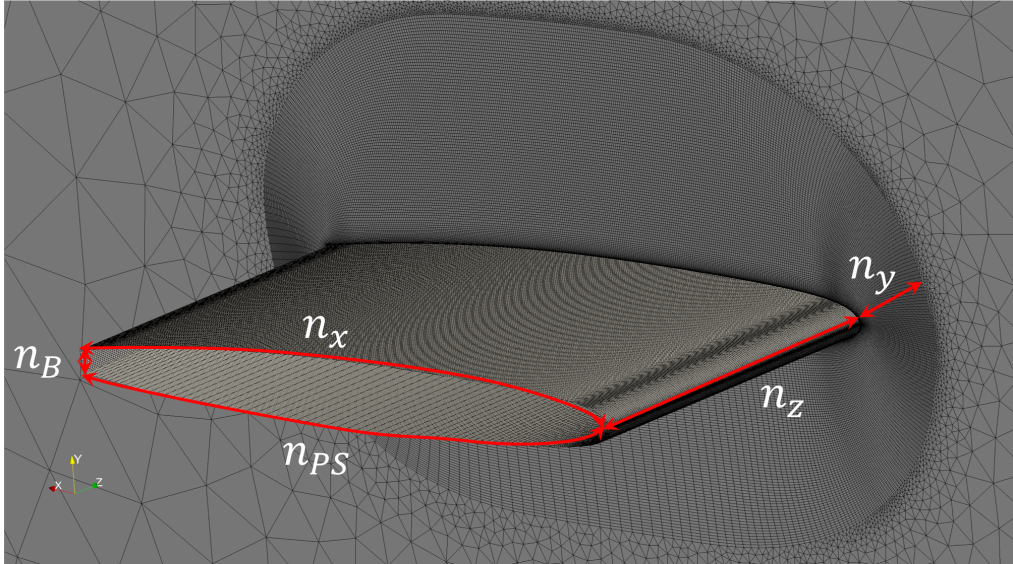
\includegraphics[width=.45\textwidth]{1.png}
\caption{Computation configuration for the foil}
\label{fig:abc}
\end{figure}
\subsubsection{Extended Framework Considerations}
An extended consideration involves a composite function $h(x) = f(g(x))$. This is purely for demonstrating nested mathematical expressions and has no theoretical basis. The comparative results of applying different placeholder functions are summarized in the double-column \tablename~\ref{tab:wide_results}.
\par
\begin{table*}[htbp]
\centering
\tablefontsize
\caption{Detailed summary of placeholder performance metrics across multiple synthetic datasets generated under varying initial parameter conditions $(\alpha, \beta, \gamma)$, including mean values $(\mu)$, standard deviations $(\sigma)$, and the computed confidence intervals $(CI_{95\%})$ for each evaluated metric (Metric A: Correlation Coefficient, Metric B: Normalized Error, Metric C: Processing Time), presented for the sole purpose of demonstrating comprehensive table formatting within a manuscript template.}
\label{tab:wide_results}
\begin{tblr}
{
columns={co=-1},
cells={valign=m,halign=c},
hline{1,Z}={wd=.08em},
hline{2}={wd=.05em},
}
Case & $x_0$ & $\alpha$ & $f(x)$        & $\sum_{i} \epsilon_i$ & $R^2$ & $T_{\text{proc}}$ (s) & Status  \\
A    & 1.0   & 0.5      & $\exp(-x)$    & 12.5                  & 0.87  & 1.2                   & Valid   \\
B    & 2.3   & 0.7      & $\log(1+x)$   & 8.9                   & 0.92  & 2.1                   & Valid   \\
C    & 0.5   & 1.2      & $x^2/(1+x^2)$ & 15.3                  & 0.75  & 0.8                   & Invalid \\
D    & 3.1   & 0.3      & $\sqrt{x}$    & 5.2                   & 0.96  & 3.0                   & Valid   \\
E    & 1.8   & 0.9      & $\sin(\pi x)$ & 22.1                  & 0.68  & 1.5                   & Invalid \\
F    & 4.0   & 0.1      & $|x-2|$       & 3.7                   & 0.98  & 4.2                   & Valid   \\
\end{tblr}
\end{table*}
\par
\section{Experimental Results and Discussion}
This section presents illustrative results generated from the aforementioned placeholder framework. The purpose is to showcase the formatting of results, figures spanning different layouts, and subsequent discussion within a template.
\subsection{Placeholder Data and Visualization}
Placeholder data was generated using a synthetic process defined by $y_i = \sin(2\pi t_i) + \epsilon_i$. This subsection describes the visualization of this data.
\subsubsection{Single-Column Figure Example}
\figurename~\ref{fig:abc} presents a schematic diagram of the placeholder process. The figure is confined to a single column to demonstrate standard figure placement and caption formatting.
\subsubsection{Double-Column Figure Example}



For broader visual comparisons, \figurename~\ref{fig:doublecol_plot} is presented across two columns. This demonstrates how wider figures can be integrated into the document layout to display more complex or detailed placeholder information in \figurename~\ref{fig:doublecol_plot:a} and \figurename~\ref{fig:doublecol_plot:f}.
\par
\begin{figure*}[htbp]
\centering
\captionsetup[subfigure]{font=footnotesize}
%\captionsetup[subfigure]{font=large}
\subcaptionbox{Condition A\label{fig:doublecol_plot:a}}{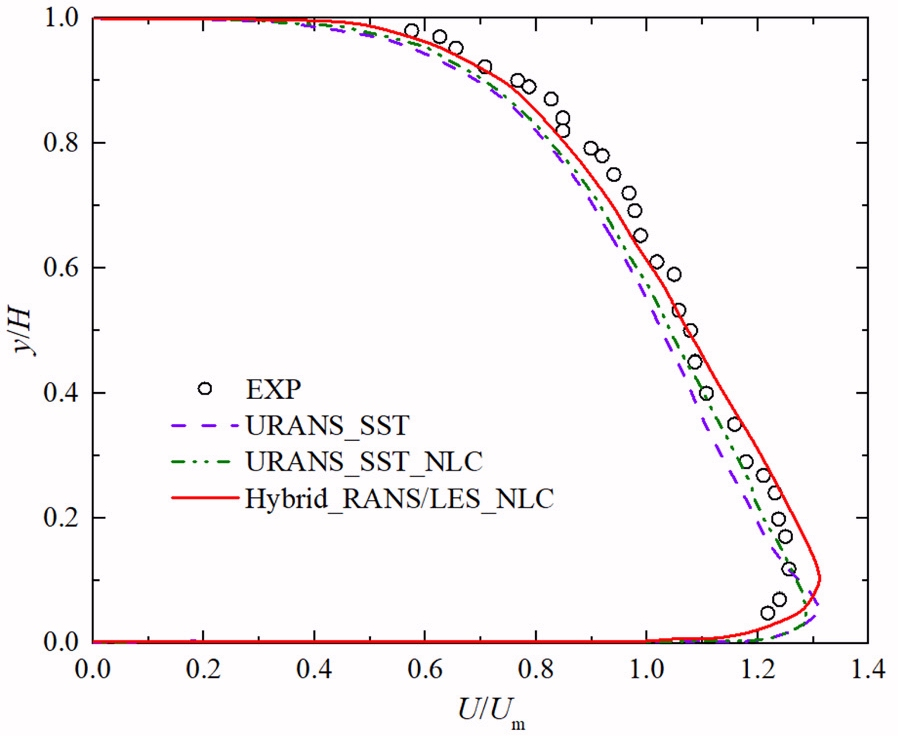
\includegraphics[width=.43\linewidth]{3a.jpg}}\hfil%
\subcaptionbox{Condition B\label{fig:doublecol_plot:b}}{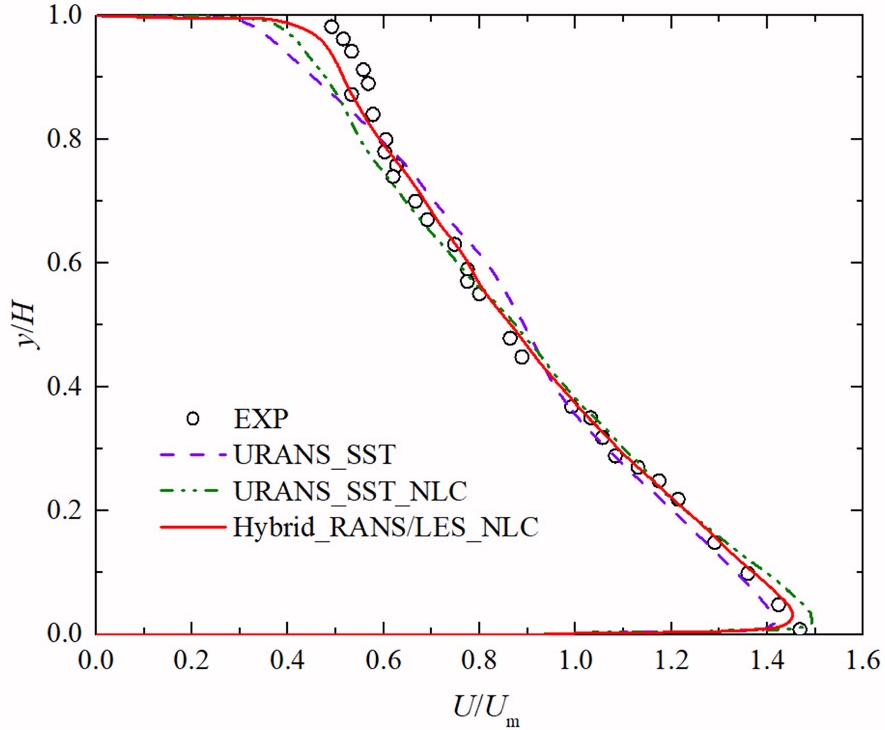
\includegraphics[width=.43\linewidth]{3b.jpg}}\hfil%
\subcaptionbox{Condition C\label{fig:doublecol_plot:c}}{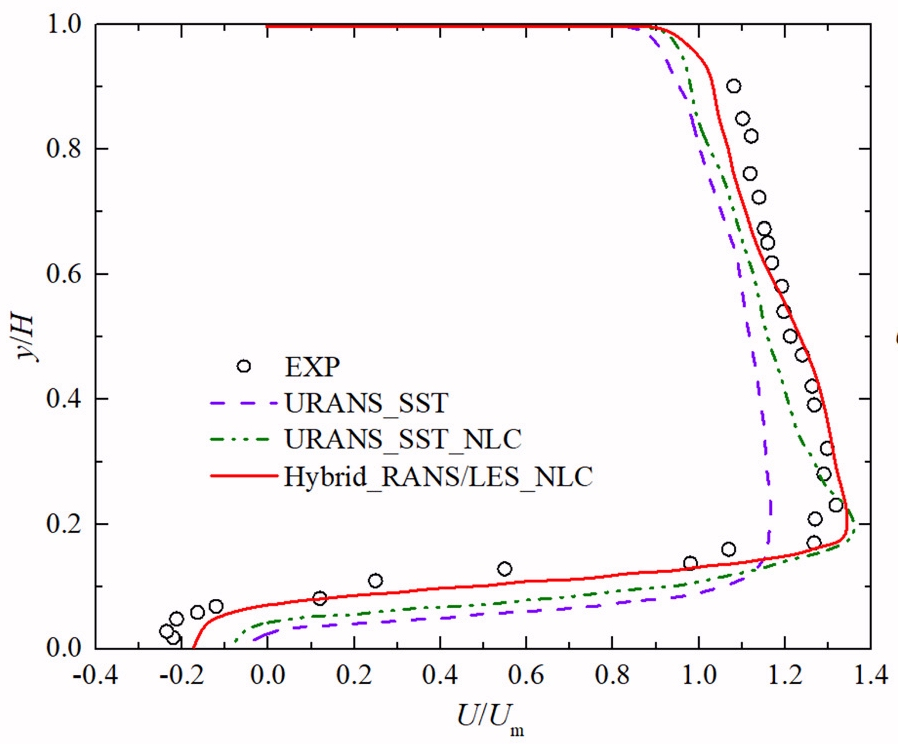
\includegraphics[width=.43\linewidth]{3c.jpg}}\hfil%
\subcaptionbox{Condition D\label{fig:doublecol_plot:d}}{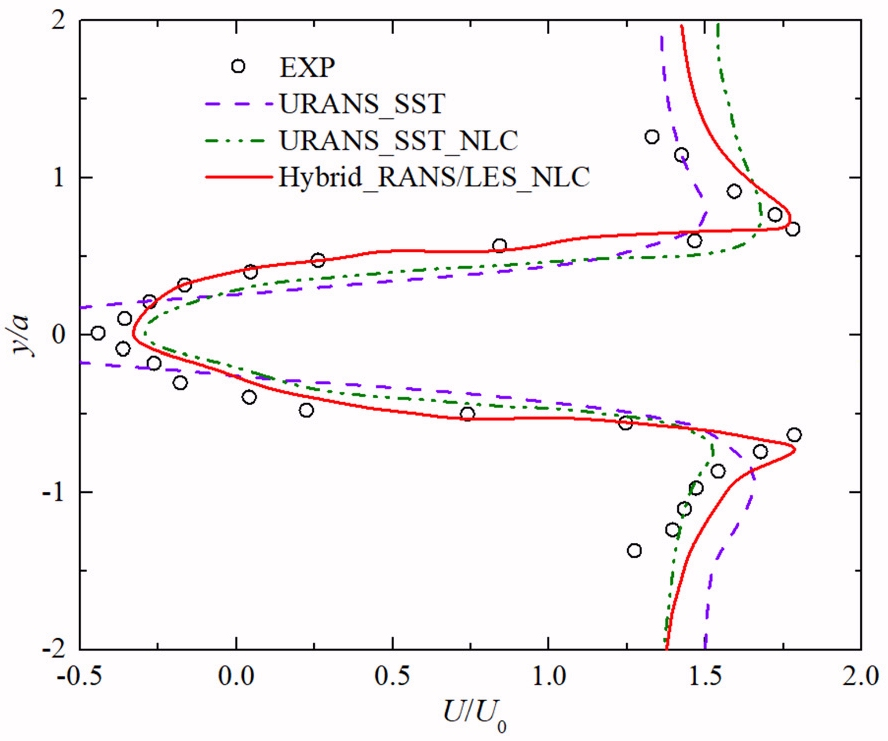
\includegraphics[width=.43\linewidth]{3d.jpg}}\hfil%
\subcaptionbox{Condition E\label{fig:doublecol_plot:e}}{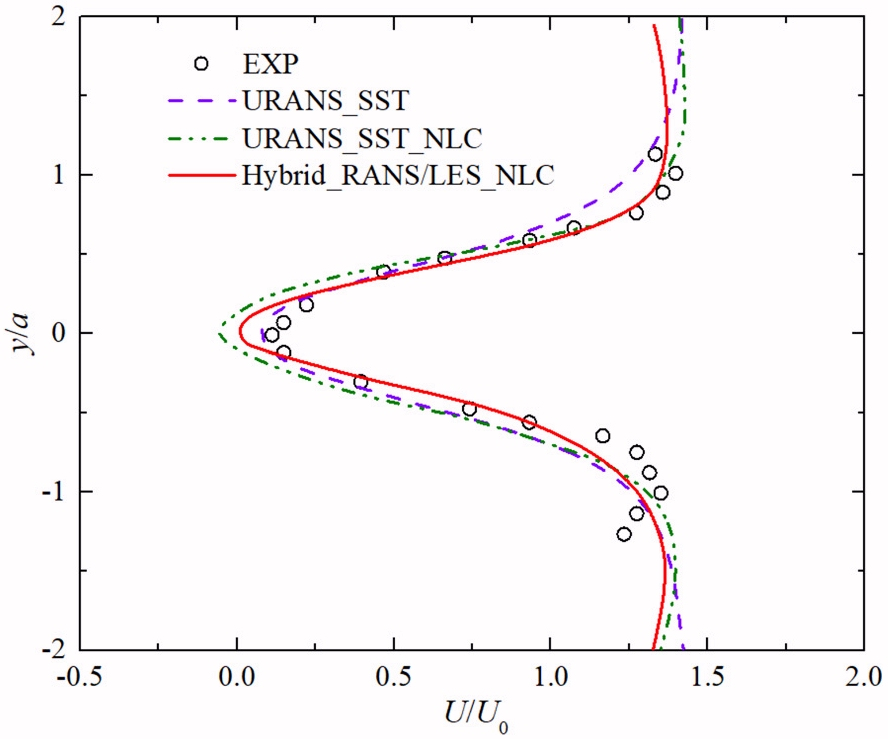
\includegraphics[width=.43\linewidth]{3e.jpg}}\hfil%
\subcaptionbox{Condition F\label{fig:doublecol_plot:f}}{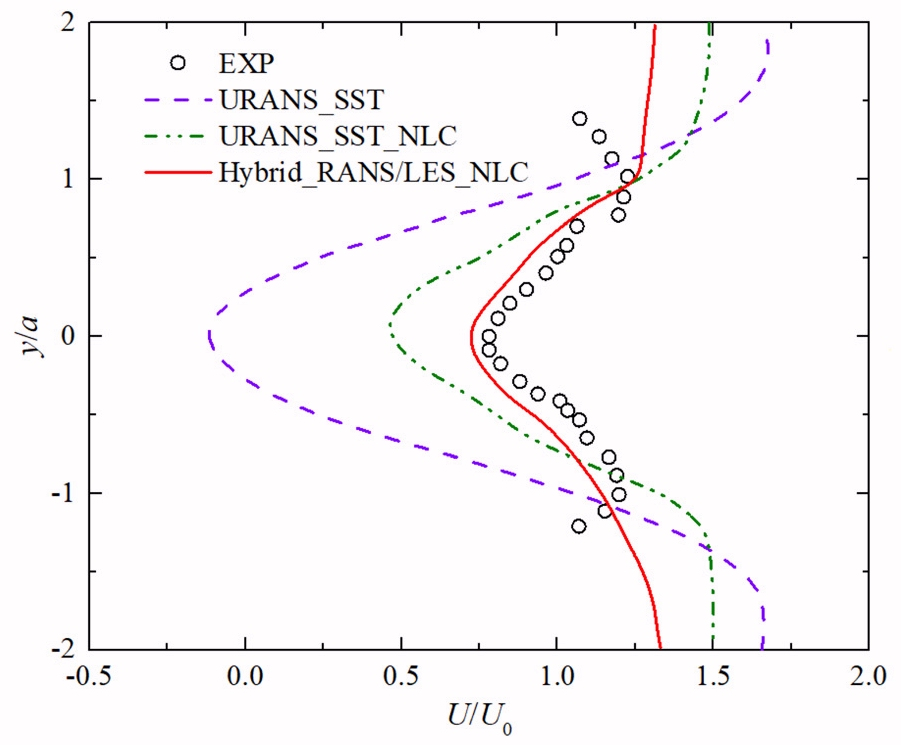
\includegraphics[width=.43\linewidth]{3f.jpg}}
\caption{Comparison of placeholder distributions across six synthetic conditions.}
\label{fig:doublecol_plot}
\end{figure*}
\par
%\begin{figure*}[htbp]
%\centering
%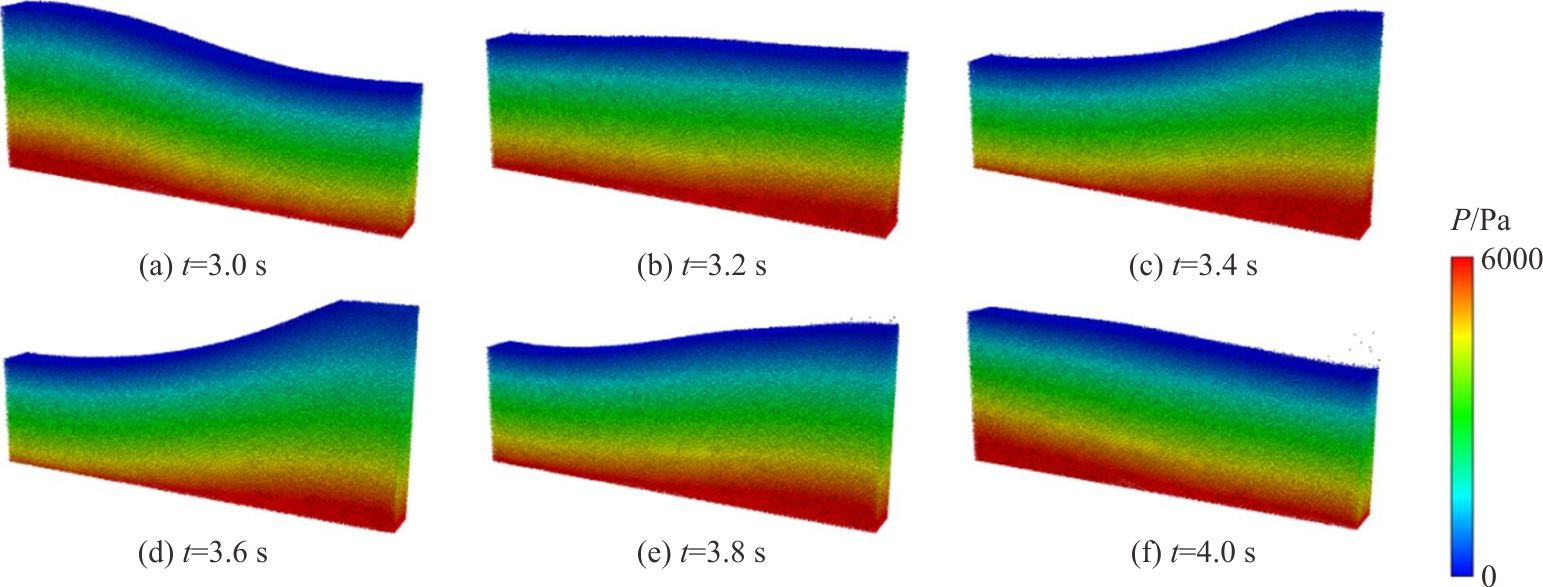
\includegraphics[width=.9\linewidth]{3.png}
%\caption{Computation configuration for the foil}
%	\label{fig:doublecol_plot1}
%\end{figure*}

\subsection{Interpretation of Placeholder Outcomes}
The outcomes, as summarized in \tablename~\ref{tab:narrow_results}, indicate no meaningful trends because all data is synthetic. The values in the table, such as those for Metric A ($\mu_A$) and Metric B ($\sigma_B$), are randomly generated for demonstration purposes only. The discussion here serves solely to exemplify how one might comment on results in a typical manuscript structure.
\par
\begin{table}[htbp]
\centering
\tablefontsize
\caption{Sample placeholder data summary.}
\label{tab:narrow_results}
\begin{tblr}
{
columns={co=-1},
cells={valign=m,halign=c},
hline{1,Z}={wd=.08em},
hline{2}={wd=.05em},
}
Parameter               & Description                 & Value           \\
$\lambda$               & Placeholder decay rate      & $0.05 \pm 0.01$ \\
$N_{\text{iter}}$       & Number of iterations        & $1000$          \\
$\sigma_{\text{noise}}$ & Standard deviation          & $0.1$           \\
$T_{\text{min}}$        & Minimum simulation time (s) & $1.0$          \\
$T_{\text{max}}$        & Maximum simulation time (s) & $10.0$          \\
\end{tblr}
\end{table}
\par
\section{Placeholder Literature Review and Citation Demonstration}
This section provides a comprehensive review of placeholder literature, aimed at demonstrating the correct formatting and integration of citations in various syntactic forms. The primary purpose is to illustrate how references to both journal articles and conference proceedings can be seamlessly woven into the narrative flow of a manuscript \cite{1,2}. This serves as a structural preview for template users, showcasing citation clustering and its visual impact within a paragraph.
\subsection{Foundational Concepts in Placeholder Studies}
The theoretical underpinnings of placeholder content generation have been explored from multiple perspectives. Early work established a basic framework for analyzing non-substantive text \cite{3}, which was later expanded upon to include systematic reviews of dummy text usage \cite{4}. A key development was the introduction of a template-based methodology \cite{5}, which significantly influenced subsequent research directions in document engineering \cite{6}. These foundational studies collectively argue for the necessity of standardized placeholder content in the publishing workflow.
\subsubsection{Structural and Visual Considerations}
Beyond mere text generation, the visual and structural integration of placeholders is critical. A comparative study on these patterns was conducted \cite{7}, while another investigation specifically focused on the role of non-meaningful text in template development \cite{8}. Their findings suggest that the spatial arrangement of elements, as much as the content itself, affects the utility of a template for preview purposes. This line of inquiry is directly relevant to the design of multi-column layouts, a topic explored in detail elsewhere \cite{6}. Furthermore, the automated approaches discussed offer promising solutions for scaling template production \cite{9}.
\subsection{Methodological Advances and Applications}
Recent years have seen significant methodological advances. The work on filler content usage \cite{10} and that on dummy reference generation \cite{11} represent practical applications of theoretical principles. Notably, a broad survey of these methodologies is provided, categorizing them by application domain \cite{12}. For instance, frameworks for citation list formatting have become increasingly sophisticated \cite{8,9}, allowing for greater customization and adherence to diverse style guides.
\subsubsection{Case Studies and Empirical Evaluations}
Empirical evaluations of these methodologies are crucial. One study evaluated the visual impact of placeholder elements, providing quantitative metrics for template effectiveness \cite{13}. Several case studies offer insights into real-world testing scenarios \cite{8}. A comparative analysis across publication formats highlights the need for adaptable placeholder strategies \cite{9}. These studies often employ the standardized approaches outlined in prior work \cite{14} and build upon established theoretical foundations \cite{15}.
\subsubsection{Integration and Future Directions}
The integration of placeholder systems into broader publishing workflows represents the current frontier. Research on template-aware citation management points towards more intelligent and context-sensitive systems \cite{10}. The collective evidence from the literature \cite{14,15,16,17,18,19,20} strongly indicates that placeholder content, while semantically empty, is structurally indispensable for the design, testing, and validation of academic manuscript templates. Future work is likely to focus on dynamic placeholder generation that adapts to specific formatting rules in real-time.
\section*{Acknowledgment}
This work was supported by XXX Foundation (Grant No. XXXXXXXX)
\section*{Conflict of interest}
All authors declare that there are no other competing interests.
\bibliography{reference}
\end{document}
